% Comandi d'intestazione, formato pagina, lingua
\documentclass[12pt,a4paper]{article}
\usepackage[utf8]{inputenc}

\setlength{\parindent}{0pt}
% Formato pagina "truccato"
\usepackage[top=2.5cm, bottom=2.5cm, left=2cm, right=2cm]{geometry}

% Palatino font
\renewcommand*\rmdefault{ppl}

%%% Pacchetti per l'ambiente matematico:
% pacchetto standard, fonts extra, simboli extra
\usepackage{amsmath}
\usepackage{amsfonts}
\usepackage{amssymb}

%%% Pacchetti di grafica
\usepackage{graphicx}
\usepackage{float}
\usepackage{adjustbox}
\usepackage{tikz}
\usepackage{forest,array}
\usetikzlibrary{shadows}

%%% Localizzazione in Italiano %%%
  \renewcommand{\figurename}{Fig.}%
  \renewcommand{\contentsname}{Indice}%
  \renewcommand{\tablename}{Tabella}%
    %~ \abstractname [only article, report]: Abstract
    %~ \appendixname: Appendix
    %~ \bibname [only book, report]: Bibliography
    %~ \chaptername [only book, report]: Chapter
    %~ \contentsname: Contents
    %~ \figurename: Figure
    %~ \indexname: Index
    %~ \listfigurename: List of Figures
    %~ \listtablename: List of Tables
    %~ \partname: Part
    %~ \refname [only article]: References
    %~ \tablename: Table
%~ \DefineBibliographyStrings{english}{%
  %~ bibliography = {Bibliografia},
  %~ references = {Riferimenti},
%~ }

% Stili per grafi
\forestset{
  giombatree/.style={
    for tree={
      grow = east,
      parent anchor=east,
      child anchor=west,
      edge={rounded corners=2mm},
      fill=violet!5,
      drop shadow,
      l sep=10mm,
      edge path={
        \noexpand\path [draw, \forestoption{edge}] (!u.parent anchor) -- +(5mm,0) -- (.child anchor)\forestoption{edge label};
      }
    }
  }
}
\forestset{
  qtree/.style={
    for tree={
      parent anchor=south,
      child anchor=north,
      align=center,
      edge={rounded corners=2mm},
      fill=violet!5,
      drop shadow,
      l sep=10mm,
    }
  }
}

\usepackage[hidelinks]{hyperref} % Nasconde link dall'indice

% PDF page in landscape
\usepackage{pdflscape}

%~ Bibliografia e citazioni
\usepackage[style=numeric,backend=bibtex]{biblatex}

\addbibresource{bibliografia.bib}

\setcounter{section}{-1}
\setcounter{secnumdepth}{5}

% Item label (pallino pieno, vuoto, trattino)
\renewcommand{\labelitemi}{$\bullet$}
\renewcommand{\labelitemii}{$\circ$}
\renewcommand{\labelitemiii}{--}

\title{Appunti di Reti Informatiche}
\author{\texttt{<giomba@live.it>} \texttt{<info@notestack.it>}}
\date{}

\begin{document}

\maketitle
\tableofcontents

\clearpage

\section{Introduzione}
Questi appunti, tratti dalle lezioni in aula del prof. Giuseppe~Anastasi,
sono da intendersi come appunti riassuntivi e, in parte, integrativi.

Questi appunti \emph{non} sono stati revisionati dal prof. Giuseppe~Anastasi.

Questi appunti potrebbero essere utili per il superamento dell'esame di
Reti Informatiche del corso di laurea triennale di Ingegneria Informatica,
ma questo non implica che siano affidabili.

L'autore non si assume nessuna responsabilità sull'uso proprio,
e specialmente improprio, che si vorrà fare di questi appunti.

Questi appunti sono stati scritti, raccolti, ampliati e ricomposti da:
\begin{itemize}
  \item giomba \texttt{<giomba@live.it>}
  \item Francesco Barbarulo {\small \texttt{<info@notestack.it>}}
\end{itemize}
che hanno fatto uso anche degli appunti di:
\begin{itemize}
  \item alex.sieni
\end{itemize}
anche se F. Barbarulo a un certo punto ha disertato :-) per cui:

Questi appunti non sono completi, perché infine sono stati scritti da
me per me, ma magari qualcun altro può comunque trovarli utili.
Per esempio, non c'è spiegato come funziona il controllo di parità,
o la firma digitale, perché lo sapevo già prima di seguire il corso.
Inoltre, disegnare le macchine a stati dei vari protocolli era
tremendamente faticoso, quindi le ho semplicemente studiate sul libro.

Ma c'è una buona notizia: il codice sorgente di questi appunti è stato
versionato con git, viene rilasciato gratuitamente sotto licenza GPL3,
e può essere consultato facendo esplicita richiesta all'autore, che
invita a ampliare, correggere e terminare il lavoro da lui incompiuto.

Buono studio!

\clearpage

\begin{landscape}
\section{Mappe}

\subsection{Argomenti generali}

\begin{center}
\begin{forest} giombatree,
[ Nodo ]
\end{forest}
\end{center}

\end{landscape}

\section{Terminologia generale}
In questa sezione vengono raccolti i termini delle reti di calcolatori,
organizzati in categorie applicative e ordinati alfabeticamente.
Vengono raccolti o solo i termini inglesi, qualora questi fossero più
diffusi, o solo i termini italiani (qualora questi fossero più diffusi,
situazione rara), o entrambe le versioni (qualora queste fossero
egualmente diffuse).

\subsection{Basi}
\begin{itemize}
  \item \textbf{access network}, rete che permette ad un host di
    collegarsi alla Internet;
  \item \textbf{client}, processo che richiede un servizio ad un server;
    per estensione, può indicare anche la macchina sulla quale tale
    processo è in esecuzione;
  \item \textbf{edge router}, il primo router che viene incontrato sul
    percorso di un pacchetto che è destinato ad un sistema collocato al
    di fuori della rete di accesso
  \item \textbf{host}, macchina collegata alla rete Internet sulla quale
    vengono eseguite delle applicazioni;
  \item \textbf{ISP}, Internet Service Provider, ente che fornisce
    connettività a Internet;
  \item \textbf{percorso} % TODO
  \item \textbf{protocollo}, insieme di regole che definiscono il formato
    e l'ordine dei messaggi scambiati tra due o più entità in
    comunicazione, e le azioni intraprese in fase di trasmissione e/o
    di ricezione di un messaggio o di un altro evento.
  \item \textbf{rete di accesso}, v. access network
  \item \textbf{RFC}, Request for Comment
  \item \textbf{route}, v. percorso
  \item \textbf{server}, processo, macchina
  \item \textbf{sistema periferico}, v. host
  \item \textbf{socket}, interfaccia
  \item \textbf{velocità di tramissione}
\end{itemize}

\subsection{Reti di accesso}
\begin{itemize}
  \item \textbf{AON}, Active Optical Network
  \item \textbf{dialup}
  \item \textbf{DSL}, SDSL, ADSL, VDSL
  \item \textbf{DSLAM}
  \item \textbf{FTTx}, FTTH, FTTC
  \item \textbf{LAN}, Local Area Network
  \item \textbf{OLT}, Optical Line Terminator
  \item \textbf{ONT}, Optical Network Terminator
  \item \textbf{PAN}, Personal Area Network
  \item \textbf{PON}, Passive Optical Network
  \item \textbf{satellite}
  \item \textbf{WAN}, Wide Area Network
  \item \textbf{WLAN}, Wireless Local Area Network
\end{itemize}

\subsection{Mezzi di trasmissione}
\begin{itemize}
  \item \textbf{cavo coassiale}
  \item \textbf{coaxial cable}, v. cavo coassiale
  \item \textbf{doppino intrecciato}
  \item \textbf{fibra ottica}
  \item \textbf{mezzo vincolato}, mezzo non vincolato
  \item \textbf{STP}, Shielded Twisted Pair
  \item \textbf{twisted pair}, v. doppino intrecciato
  \item \textbf{UTP}, Unshielded Twisted Pair
\end{itemize}

\subsection{Network Core, Nucleo della Rete}
\begin{itemize}
  \item \textbf{ampiezza di banda}
  \item \textbf{bandwidth}, v. ampiezza di banda
  \item \textbf{circuit switching}
  \item \textbf{commutazione di circuito}, v. circuit switching
  \item \textbf{commutazione di pacchetto}
  \item \textbf{FDM}, Frequency Division Multiplexing
  \item \textbf{pacchetto}
  \item \textbf{packet}, v. pacchetto
  \item \textbf{packet loss}
  \item \textbf{packet switching}, v. commutazione di pacchetto
  \item \textbf{perdita di pacchetto}, v. packet loss
  \item \textbf{store and forward}
  \item \textbf{TDM}, Time Division Multiplexing
\end{itemize}

\subsubsection{TDM}
\begin{itemize}
  \item \textbf{frame}
  \item \textbf{slot}
\end{itemize}

\subsubsection{FDM}
\begin{itemize}
  \item \textbf{portante}
\end{itemize}

\subsection{ISP}
\begin{itemize}
  \item \textbf{ISP di accesso}
  \item \textbf{ISP di livello \#}
  \item \textbf{ISP regionale}
  \item \textbf{IXP}, Internet Exchange Point, punto d'incontro in cui
    più ISP possono fare peering tra loro
  \item \textbf{peering}, interconnessione di reti di ISP di pari
    livello, al fine di ridurre i costi per l'attraversamento delle
    reti di ISP di livello superiore
  \item \textbf{tier-\# ISP}, v. ISP di livello \#
\end{itemize}

\subsection{Ritardi nelle reti packet switching}
\begin{itemize}
  \item \textbf{di accodamento}
  \item \textbf{di elaborazione}
  \item \textbf{di propagazione}
  \item \textbf{di trasmissione}
  \item \textbf{RTT}, Round Trip Time
\end{itemize}

\subsection{Velocità di trasmissione}
\begin{itemize}
  \item \textbf{throughput}
  \item \textbf{collo di bottiglia}
\end{itemize}

\subsection{Architettura a livelli}
\begin{itemize}
  \item \textbf{applicazione}
  \item \textbf{collegamento}
  \item \textbf{fisico}
  \item \textbf{rete}
  \item \textbf{trasporto}
\end{itemize}

\section{Livello di Applicazione}
\begin{table}[H]
  \centering
  \begin{tabular}{| c | c | c | c | c |}\hline
  Protocollo  & Porta & Trasporto & Persistenza         & Stato \\ \hline
  HTTP        & 80    & TCP       & sì/no               & no    \\ \hline
  FTP         & 21    & TCP       & sì comandi; no dati & sì    \\ \hline
  SMTP        & 25    & TCP       & sì                  & sì    \\ \hline
  POP         & 110   & TCP       & sì                  & sì    \\ \hline
  IMAP        & 143   & TCP       & sì                  & sì    \\ \hline
  DNS         & 53    & UDP       & --                  & no    \\ \hline
  \end{tabular}
  \caption{Tabella comparativa tra alcuni protocolli di livello applicazione}
\end{table}

\subsection{FTP, File Transfer Protocol}
Il protocollo prevede la presenza di un canale di comunicazione per i
comandi, creato all'inizio della sessione, e di uno o più canali per il
trasferimento di dati vero e proprio, creati all'occorrenza.

\subsubsection{Funzionamento}
\begin{enumerate}
  \item Il client apre una connessione verso il server sulla porta~21,
    ed esegue l'autenticazione con nome utente e password; è anche
    possibile una connessione anonima;
  \item Il client richiede un file (oppure il listing dei file) inviando
    un apposito comando sulla connessione;
  \item Il server acconsente al trasferimento delle informazioni aprendo
    una nuova connessione verso il client e inviando i dati attraverso
    di essa; quando tutti i dati sono stati trasmessi, la connessione
    viene chiusa;
\end{enumerate}

Mentre avviene un trasferimento di dati, il client può comunque eseguire
altre operazioni sul server tramite la connessione per i comandi: per
esempio può richiedere un nuovo file, può richiedere di inviare un nuovo
file, può navigare nell'albero del filesystem e richiedere il listato di
altre directory.

\subsection{DNS, Domain Name System}
\begin{forest} qtree,
[ Root DNS Servers
  [ TLD .it Servers
    [ DNS Server\\ notestack.it ]
    [ DNS Server\\ giomba.it ]
    [ ... ]
  ]
  [ TLD .org
    [ DNS Server\\ altervista.org ]
    [ DNS Server\\ ils.org ]
    [ ... ]
  ]
  [ TLD ... ]
]
\end{forest}

\begin{itemize}
  \item \textbf{root DNS server}
  \item \textbf{TLD server}
  \item \textbf{authoritative server}
\end{itemize}

\begin{itemize}
  \item \textbf{Approccio iterativo}
  \item \textbf{Approccio ricorsivo}
\end{itemize}

\subsubsection{Record DNS}
\texttt{ (type, name, value, TTL) }

\begin{table}[H]
  \centering
  \begin{tabular}{| c | c | c |}\hline
    Type      & Name      & Value                           \\ \hline
    A, AAAA   & hostname  & IP address                      \\ \hline
    NS        & domain    & authoritative server hostname   \\ \hline
    CNAME     & alias     & hostname                        \\ \hline
    MX        & alias     & hostname                        \\ \hline
  \end{tabular}
  \caption{Significato dei campi dei record DNS in base ad alcuni tipi}
\end{table}

\subsubsection{Messaggio DNS}
\begin{verbatim}
  struct DNS_Message_hdr {
    uint16_t id;
    uint16_t flag;
    uint16_t n_domande;
    uint16_t n_risposte;
    uint16_t n_autoritativi;
    uint16_t n_addizionali;
  };
\end{verbatim}
Seguito dal rispettivo numero di campi indicato nell'intestazione.

\subsubsection{Inserimento di record nel database DNS}
Esempio di inserimento di example.org nel database.

\begin{enumerate}
  \item
    Posseggo l'organizzazione \emph{Example}; voglio avere un sito web \emph{www.example.org}.
    Chiedo al registrar di primo livello per il dominio .org se il nome \emph{example} è disponibile.
    Se è disponibile, allora procedo.
  \item
    Mi procuro un server DNS: il suo hostname sarà dns1.example.org; il suo indirizzo IP è 192.0.2.1.
    Contatto il registrar chiedendo
    di registrare il nome example; comunico anche i dati del mio server DNS autoritativo.
  \item Il registrar inserisce nel suo database i seguenti record:
    \begin{verbatim}
      ( A,  dns1.example.org, 192.0.2.1        )
      ( NS, example.org,      dns1.example.org )
    \end{verbatim}
  \item
    Mi procuro un server web: il suo hostname è webserver1.example.org; il suo indirizzo IP è 192.0.2.2.
    Inserisco nel mio server DNS autoritativo i seguenti record:
    \begin{verbatim}
      ( A,     webserver1.example.org, 192.0.2.2              )
      ( CNAME, www.example.org,        webserver1.example.org )
    \end{verbatim}
\end{enumerate}

Per curiosità, la rete 192.0.2.0/24 è una rete dedicata alla documentazione
di esempio, come definito nell'RFC~5737.

\subsection{BitTorrent}
\subsubsection{Terminologia}
\begin{itemize}
  \item \textbf{chunk}, pezzo di file: un file viene scomposto in tanti
    chunk di dimensione fissa (es. 256~kiB -- 2~MiB);
  \item \textbf{freerider}, peer che partecipa ad un torrent solo per
    ottenere chunk e non per condividerli con altri peer; un freerider
    adotta un comportamento antietico e viene penalizzato dai peer
    che implementano correttamente il protocollo;
  \item \textbf{leecher}, utente che partecipa onestamente ad un torrent
    per ottenere chunk per il file di cui ha bisogno;
  \item \textbf{rarest first}, comportamento che indica che i peer si
    scambiano i chunk dando precedenza a quelli più più rari;
  \item \textbf{seeder}, peer che ha completato lo scaricamento di un
    file e, altruisticamente, rimane nel torrent per condividere i chunk
    in suo possesso;
  \item \textbf{torrent}, insieme di peer che partecipa alla
    condivisione di un file;
  \item \textbf{tracker}, server dedicato a tenere traccia dei peer
    appartenenti ad un torrent di un file;
\end{itemize}

\subsubsection{Funzionamento}
\begin{enumerate}
  \item Un peer X si procura un file \emph{.torrent} attraverso un
    motore di ricerca: nel file sono presenti informazioni circa i
    \emph{tracker} che tengono traccia dello stato dei peer
    appartenenti a quel torrent.
  \item X sceglie un tracker e annuncia la sua intenzione di
    partecipare al torrent di un determinato file; il tracker gli
    fornisce una lista, sottoinsieme dei peer che stanno partecipando
    al torrent; i peer di questa lista vengono detti \emph{vicini} di X;
    X diventa un \emph{leecher};
  \item Il peer interroga i suoi vicini, ottenendo
    informazioni sui chunk che ognuno di essi possiede; stabilito quali
    siano i chunk più rari, li richiede ai vicini che li posseggono;
  \item Prima o poi, gli altri vicini risponderanno alle richieste e
    invieranno i loro chunk. X stabilisce quali vicini gli stanno
    inviando dati a maggiore velocità, li inserisce in una lista di
    preferiti\footnote{le specifiche del protocollo definiscono questi
    vicini come \emph{unchoked} o \emph{non soffocati}, in contrasto
    con tutti gli altri che invece sono \emph{choked}, \emph{soffocati}}
    e ricambia il favore fornendo loro i chunk di cui è in possesso e
    che gli sono stati richiesti;
  \item Periodicamente, X sceglie un vicino casuale e inizia a inviargli
    i chunk da esso richiesti, nella speranza che questo ricambi
    inviandogli i suoi chunk ad una velocità maggiore degli altri;
    contemporaneamente, elimina un vicino dalla sua lista di peer
    preferiti.
  \item Quando X ha ottenuto tutti i chunk di un file, può rimanere nel
    torrent, offrendo i suoi chunk agli altri peer e divenendo così un
    \emph{seeder}, oppure può uscire dal torrent, divenendo una
    TdC\footnote{questo non è definito dal protocollo}.
\end{enumerate}

Da questo comportamento segue che:
\begin{itemize}
  \item ogni peer si accoppia sempre con altri peer che hanno velocità
    paragonabili alla propria;
  \item i freerider, non condividendo chunk con altri peer, sono
    penalizzati in quanto vengono tolti dalle liste di preferenza più
    frequentemente rispetto ai peer onesti;
  \item i chunk più rari vengoni condivisi con maggiore frequenza, così
    la concentrazione dei vari chunk tende a rimanere omogenea nel
    tempo;
\end{itemize}

\subsection{Considerazioni sui modelli client-server e peer-to-peer}
Vogliamo minimizzare il tempo di distribuzione di un file in funzione
del numero di client.

Ipotesi:
\begin{itemize}
  \item Il bottleneck è determinato dai collegamenti di accesso di
    client e server, in quanto la rete Internet ha banda a sufficienza;
  \item siano $d_s$, $u_s$ i bitrate, rispettivamente in download e
    in upload, del server;
  \item siano $d_i$, $u_i$ i bitrate, rispettivamente in download e
    in upload, del client $i$
  \item sia $N$ il numero di client
  \item sia $L$ la dimensione del file
\end{itemize}

\begin{table}[H]
\centering
\begin{tabular}{| p{10cm} | c |}\hline
  Il server deve trasmettere il file per $N$ volte  & $\frac{N L}{u_s} $ \\ \hline
  Il client più lento deve ricevere il file         & $\frac{L}{\min_{i}(d_i)} $ \\ \hline
\end{tabular}
\caption{Tempi minimi di distribuzione per modello client-server}
\label{tab:tempi-cs}
\end{table}

\begin{table}[H]
\centering
\begin{tabular}{| p{10cm} | c |}\hline
  Il server deve trasmettere il file almeno una volta & $\frac{L}{u_s}$ \\ \hline
  Il client più lento deve ricevere il file           & $\frac{L}{\min_{i}(d_i)}$ \\ \hline
  Il file deve essere trasmesso almeno per $N$ volte
  tramite la capacità di upload dell'intero sistema   & $\frac{N L}{u_s + \sum_{i} u_i}$ \\ \hline
\end{tabular}
\caption{Tempi minimi di distribuzione per modello peer-to-peer}
\label{tab:tempi-p2p}
\end{table}

I tempi minimi di distribuzione del modello client-server e del modello
peer-to-peer sono quindi dati dal massimo tra i termini evidenziati,
rispettivamente, nella Tabella~\ref{tab:tempi-cs} e nella
Tabella~\ref{tab:tempi-p2p}.

I termini più rilevanti sono:

$$ t_{CS} = \frac{N L}{u_s + \sum_{i} u_i} $$
$$ t_{P2P} = \frac{N L}{u_s} $$

Perciò è facilmente dimostrabile che, se si considera con buona
approssimazione $u_i = u_c = cost ~ \forall i$ (tutti i client hanno la
stessa velocità in upload) all'aumentare di $N$, $t_{CS}$ aumenta
linearmente, mentre $t_{P2P}$ tende ad un valore costante.

$$ \lim_{N\to\infty} t_{CS} = \infty $$
$$ \lim_{N\to\infty} t_{P2P} = \lim_{N\to\infty} \frac{N L}{u_s + N u_c} = \lim_{N\to\infty} \frac{N L}{N (u_c + \frac{u_s}{N}) } = \frac{L}{u_c} $$

\section{Livello di Collegamento}
\begin{landscape}

\begin{forest} giombatree,
[ Collegamento
  [ Error
    [ Detection
      [ Parity Check ]
      [ Checksum ]
      [ CRC ]
    ]
    [ Correction
      [ Matrix Parity Check ]
    ]
  ]
  [ Reliable Data Transfer
    [ Stop-and-wait ]
    [ Pipelining
      [ Go-back-N ]
      [ Selective Repeat ]
    ]
  ]
  [ Protocolli
    [ accesso multiplo
      [ Suddivisione Canale
        [ TDMA ]
        [ FDMA ]
        [ CDMA ]
      ]
      [ Accesso Casuale
        [ ALOHA Slotted ]
        [ ALOHA Puro ]
        [ CSMA/CD ]
      ]
      [ A rotazione
        [ polling ]
        [ con Token ]
      ]
    ]
    [ point-to-point
      [ PPP ]
    ]
  ]
  [ Ethernet ]
  [ ATM ]
]
\end{forest}
\end{landscape}

\subsection{Terminologia}
\begin{itemize}
  \item \textbf{collegamento}
  \item \textbf{MAC}, Medium Access Control
  \item \textbf{NIC}, Network Interface Card
  \item \textbf{framing} incapsulamento dei dati da trasmettere in una \emph{trama},
    costituita da una intestazione (header), da un epilogo (trailer) e dai
    dati effettivi da trasmettere (payload).\\
    \begin{tabular}{| c | c | c |} \hline
      Header & ~~~~~~~~~Payload~~~~~~~~~ & Trailer \\ \hline
    \end{tabular}
\end{itemize}

\subsection{Error Detection and Correction}
\subsubsection{Error Detection}
\paragraph{Parity Check}
\paragraph{Checksum}
\paragraph{CRC, Cyclic redundancy check}

\subsubsection{Error Correction}
\begin{itemize}
  \item \textbf{FEC}, Forward Error Correction, capacità del ricevente
    di individuare la presenza di errori e di correggerli (entro determinati
    limiti)
\end{itemize}
\paragraph{Matrix Parity Check}

\subsection{Protocolli point-to-point}
\subsubsection{PPP}
\begin{itemize}
  \item Cosa fa:
  \begin{itemize}
    \item trasporto dati a livello di collegamento e a livello di rete
    \item error detection
    \item controlla attività della connessione
    \item negoziazione indirizzi a livello di rete
  \end{itemize}
  \item Cosa non fa:
  \begin{itemize}
    \item error correction
    \item consegna in ordine
    \item controllo di flusso
    \item supporto multipunto
  \end{itemize}
\end{itemize}

\paragraph{Frame PPP}\mbox{}\\
\begin{table}[H]
  \centering
  \begin{tabular}{| c | c | c | c | c | c | c |} \hline
    FLAGS    & ADDRESS  & CONTROL & PROTOCOL    & DATA        & CHECK     & FLAGS    \\ \hline
    01111110 & unused   & unused  & dest. level & actual data & redudancy & 01111110 \\ \hline
  \end{tabular}
  \caption{Frame PPP}
\end{table}

\paragraph{Byte stuffing / unstuffing}\mbox{}\\
In fase di trasmissione, nel campo \emph{data} viene inserito un byte di
escape prima di ogni byte identico ai byte di header e trailer, e prima
di ogni byte identico al byte di escape.

In fase di ricezione, quando si riceve un byte di escape si scarta, mentre
si mantiene il byte immediatamente successivo.

\subsection{Protocolli ad accesso multiplo}
\begin{itemize}
  \item \textbf{collisione} condizione di errore in cui più nodi trasmettono
  sul nodo, rendendo in tal modo impossibile la decodifica da parte dei
  ricevitori
\end{itemize}

\subsubsection{Criteri di classificazione dei protocolli ad accesso multiplo}
Classificazione dei protocolli ad accesso multiplo tramite i seguenti criteri:
\begin{itemize}
  \item \textbf{utilizzazione totale}
  \item \textbf{imparzialità}, o fairness
  \item \textbf{decentralizzato}
  \item \textbf{KISS}, Keep It Simple Stupid
\end{itemize}

\begin{table}[H]
  \centering
  \begin{tabular}{| c | c | c | c | c |}
  \hline
  Protocol    & Full utilization? & Fair? & Centralized?  & Simple? \\ \hline
  TDMA        & no                & yes   & yes           & yes     \\ \hline
  FDMA        & no                & yes   & yes           & yes     \\ \hline
  CDMA        & yes               & yes   & yes           & no      \\ \hline
  ALOHA slot  & yes               & ??    & yes           & --      \\ \hline
  ALOHA pure  & yes               & ??    & no            & yes     \\ \hline
  CSMA        & yes               & ??    & no            & no      \\ \hline
  Polling     & yes               & ??    & yes           & yes     \\ \hline
  Token       & yes               & no    & yes           & yes     \\ \hline
  %~ ...         & ...               & ...   & ...           & ...     \\ \hline
  % to be continued
  \end{tabular}
  \caption{Tabella comparativa di alcuni protocolli ad accesso multiplo}
\end{table}

\subsubsection{Divisione del canale}
\paragraph{TDMA}
  Time Division Multiple Access: ad ogni nodo viene assegnato uno slot
  temporale predefinito, in cui può occupare il mezzo per tutta la sua
  ampiezza di banda.
\paragraph{FDMA}
  Frequency Division Multiple Access: ad ogni nodo viene assegnata una
  parte della banda del mezzo, che può occupare per trasmettere.
\paragraph{CDMA}\mbox{}\\
  Code Division Multiple Access: ad ogni coppia di nodi viene assegnato
  un codice, con i quali i due nodi "codificano" i dati da scambiarsi.
  La conoscenza del codice permette ai ricevitori di decodificare
  solamente le trame a loro destinati, distinguendole da quelle
  codificate con un codice diverso. Analogia umana: parlo in italiano
  con un mio amico mentre contemporaneamente degli stranieri mi parlano
  accanto (per me è solo rumore incomprensibile).
\subsubsection{Accesso casuale}
\paragraph{ALOHA Slotted}\mbox{}\\
Il tempo viene suddiviso in slot.
La durata di uno slot è sufficiente per la trasmissione di un pacchetto
e per la ricezione del suo ACK.

Quando un nodo ha un pacchetto da trasmettere, attende l'inizio del
primo slot in ordine temporale, quindi trasmette il pacchetto.

Se non riceve l'ACK, allora: si attende l'inizio dello slot successivo,
e si ritrasmette il pacchetto con probabilità \emph{p}.

\subparagraph{Massima utilizzazione}\mbox{}\\
Dati $N$ nodi, la probabilità di successo della trasmissione di un nodo
in un determinato slot è $p(1-p)^{N-1}$, perciò la probabilità che lo
slot venga utilizzato in maniera utile è $P_{SUCC} = Np(1-p)^{N-1}$.
\\ \\
Fissato $N$, qual è il valore di $p$ per cui $P_{SUCC}$ è massima?
$$ \frac{\partial}{\partial p} Np(1-p)^{N-1} = 0 \implies p = \frac{1}{N} $$

Noto quindi $p$, qual è la probabilità di successo all'aumentare dei nodi?
$$ \lim_{N\to\infty} \left(1-\frac{1}{N}\right)^{N-1} = \frac{1}{e} \approx 0.37 $$

\paragraph{ALOHA Unslotted}
Analogo ad ALOHA~Unslotted, con l'unica differenza che il tempo non è
suddiviso in slot. La trasmissione del pacchetto inizia non appena
questo è pronto, senza dover aspettare il primo slot in ordine
temporale.

\subparagraph{Massima utilizzazione}\mbox{}\\
Dati $N$ nodi, la probabilità di successo della trasmissione di un nodo
è $p(1-p)^{N-1}(1-p)^{N-1}$: nell'intervallo di tempo corrispondente
allo slot, il tal nodo deve trasmettere, mentre tutti gli altri nodi
non devono iniziare la trasmissione negli intervalli temporali, di
durata di uno slot, immediatamente precedenti e immediatamente
successivi alla trasmissione. La probabilità che un intervallo temporale
venga utilizzato in maniera utile è
$P_{SUCC} = Np(1-p)^{2(N-1)} $.
\\ \\
Fissato $N$, qual è il valore di $p$ per cui $P_{SUCC}$ è massima?
$$ \frac{\partial}{\partial p} Np(1-p)^{2(N-1)} = 0 \implies p = \frac{1}{2N-1}$$

Noto quindi $p$, qual è la probabilità di successo all'aumentare dei nodi?
$$ \lim_{N\to\infty} N\left(\frac{1}{2N-1}\right)\left(1-\frac{1}{2N-1}\right)^{2(N-1)} = \frac{1}{2e} \approx 0.18 $$

Osservazione elementare: ALOHA slotted è doppiamente migliore di ALOHA puro.

\paragraph{CSMA e CSMA/CD}\mbox{}\\
\begin{itemize}
  \item \textbf{Carrier Sense Multiple Access}: prima di trasmettere un
  pacchetto, il nodo controlla che sul mezzo trasmissivo non sia già in
  corso un'altra trasmissione. Se il mezzo è occupato, allora il nodo
  attende un tempo casuale prima di ripetere la verifica (e
  trasmettere, in caso di esito positivo). Le collisioni possono
  comunque verificarsi perché un nodo potrebbe non percepire che il
  mezzo è occupato nel caso in cui i ritardi di propagazione siano
  rilevanti. Una volta che la trasmissione di un pacchetto è iniziata,
  viene comunque sempre portata a termine.
  \item \textbf{CSMA/Collision Detection}: analogo a CSMA, ma in
  aggiunta il nodo trasmettitore rimane in ascolto del mezzo anche
  durante la trasmissione, e, se rileva una collisione, la interrompe,
  limitando lo spreco di tempo.
\end{itemize}
\subsubsection{A turno}
\paragraph{Tipo polling}\mbox{}\\
Nella rete viene identificato un modo master che, a rotazione, invita i
client a trasmettere, dando loro il permesso di occupare il mezzo. Un
nodo trasmette sul bus solo quando riceve l'invito esplicito dal
master.

Se il master si guasta, dopo un po' i nodi possono scegliere un nuovo
master tramite un algoritmo di elezione.

\paragraph{Tipo token}\mbox{}\\
La rete è generalmente organizzata ad anello. Nella rete esiste un
pacchetto particolare detto \emph{token} (testimone). Ogni nodo può
trasmettere solo quando possiede il token.

Un nodo A che ha ricevuto il token trasmette i pacchetti sul mezzo verso
un nodo B adiacente. B ritrasmette il pacchetto al suo nodo adiacente C,
e così via.
Se un nodo è destinatario del pacchetto, prima di trasmetterlo lo copia
nella sua memoria locale.
Quando il pacchetto ha terminato il giro dell'anello, ritorna al nodo di
origine A, e tale evento funge da ACK.
Quindi il nodo di origine, se non ha altri pacchetti da trasmettere,
trasmette il pacchetto token al suo nodo adiacente B.

\subsection{Protocollo Ethernet}
Ethernet è pensato per funzionare con reti con topologia a stella e a
bus. Ethernet definisce sia il protocollo a livello di collegamento,
sia alcune specifiche a livello fisico.

\subsubsection{Frame Ethernet}
\begin{table}[H]
  \centering
  \begin{tabular}{| c | c | c | c | c | c |}\hline
  Preamble  & dst. addr.  & src. addr.  & Type  & Data    & CRC \\ \hline
  8         & 6           & 6           & 2     & 46-1500 & 4   \\ \hline
  \end{tabular}

  \begin{tabular}{| c | c |}\hline
    Field       & Notes                                   \\ \hline
    preamble    & \texttt{10101010} $ \times $ 7 + \texttt{10101011} $ \times $ 1   \\ \hline
    dst. addr.  & Destination MAC Address                 \\ \hline
    src. addr.  & Source MAC Address                      \\ \hline
    type        & Level-3 protocol destination            \\ \hline
    data        & Actual data                             \\ \hline
    CRC         & Cyclic Redudancy Check                  \\ \hline
  \end{tabular}
  \caption{Frame Ethernet}
\end{table}

\begin{itemize}
  \item preamble: preambolo utilizzato a livello fisico per sincronizzare
    il ricevitore sul clock del trasmettitore. Server per la codifica Manchester.
  \item dst. addr: MAC address della NIC destinataria; \texttt{0xFF.FF.FF.FF.FF.FF}
    per il broadcast
  \item src. addr: MAC address della NIC mittente
  \item type: indica a quale protocollo di livello di rete devono essere
    consegnati i dati trasmessi (es. IP)
  \item data: i dati effettivi da trasmettere
  \item CRC: ridondanza di controllo
\end{itemize}

\paragraph{Codifica Manchester}\mbox{}\\
I due segnali di clock e dati vengono trasmessi contemporaneamente:
$S_{tot} = b_{i}$ xor $clock$

\paragraph{Considerazioni sulla dimensione del frame}\mbox{}\\
La minima dimensione del frame è di 64~bytes. Infatti siano:

\begin{itemize}
  \item $l$ lunghezza massima del link (2500 m)
  \item $v$ velocità di propagazione del segnale elettrico nel mezzo
  \item $L$ lunghezza del frame
  \item $R$ velocità di trasmissione dei dati nel mezzo
\end{itemize}

allora, il tempo $\tau $ di propagazione del segnale è:

$$ \tau = \frac{l}{v} $$

e il tempo $ t_{TX} $ per trasmettere un pacchetto è:

$$ t_{TX} = \frac{L}{R} $$

Affinché una NIC ad una estremità del bus possa accorgersi che la trama
che sta trasmettendo sta generando una collisione, nel caso peggiore in
cui una NIC all'altra estremità inizi la trasmissione nel momento esatto
in cui riceve la trama della prima NIC, $ t_{TX} > \tau $, quindi:

$$ L > \frac{2 l R}{v} $$

cioè 64 bytes.

\subsubsection{Topologie}
\begin{itemize}
  \item \textbf{dominio di collisione}: insieme di nodi collegato ad un
    mezzo condiviso per i quali si può verificare una collisione
  \item \textbf{dominio di broadcast}: insieme di nodi raggiugibili da
    un frame broadcast Ethernet
\end{itemize}

L'estensione dei domini di collisione dipende sia dalla topologia della
rete (bus o stella), sia dai dispositivi utilizzati per realizzarla.

\begin{itemize}
  \item \textbf{hub}: dispositivo centrale per una rete a stella,
    operante a livello fisico. Un hub vede solo i segnali elettrici.
    Tutti i nodi collegati ad un hub appartengono allo stesso dominio di
    collisione. Oggi rimpiazzato da switch.
  \item \textbf{switch}: dispositivo centrale per una rete a stella,
    operante a livello di collegamento. Inoltra i pacchetti in modo
    "intelligente". Separa i domini di collisione.
\end{itemize}

\subsubsection{CSMA/CD Ethernet}
Protocollo CSMA/CD utilizzato in Ethernet.

\begin{enumerate}
  \item La NIC attende che il canale rimanga libero per il tempo
    necessario a trasmettere almeno 96bit a 10Mbps (9.6 $\mu$s)
  \item La NIC trasmette. Se non si verifica nessuna collisione, allora
    il frame si considera trasmesso e ricevuto correttamente.
  \item Se viene rilevata una collisione, la NIC interrompe la
    trasmissione e invia il \emph{segnale di jam}; quindi attende un
    tempo casuale di \emph{backoff} e ritenta la trasmissione dal
    punto~1.
\end{enumerate}

\paragraph{Algoritmo di backoff}

Viene scelto un numero casuale $k$ in un insieme di numeri.

\begin{table}[H]
  \centering
  \begin{tabular}{ l l }
    Collisione 1          & $ k \in [0, 1] $        \\
    Collisione 2          & $ k \in [0, 1, 2, 3] $  \\
    ...                   & ...                     \\
    Collisione $n$-esima  & $ k \in [0, 2^n - 1] $  \\
  \end{tabular}
  \caption{Scelta di $k$ nell'algoritmo di backoff}
\end{table}

Tempo di backoff $ \beta $: $ \beta = k \times 51.2 \mu s $

\begin{itemize}
  \item Dalla decima collisione in poi $ k \in [0, 2^{10} - 1] $
  \item Alla 17esima collisione di fila, la trasmissione viene abortita
\end{itemize}

\paragraph{Segnale di jam}
48 bit trasmessi a potenza maggiorata, così che tutti i nodi possano
capire che si è verificata una collisione.

\subsubsection{Standard Ethernet a livello fisico}
In Ethernet il protocollo di livello di collegamento è indipendente
dallo specifico mezzo fisico utilizzato, perciò può funzionare con cavi
coassiali, doppini intrecciati, fibra ottica.

10BASE-5
\begin{itemize}
  \item \texttt{\^{}[0-9]*} indica la velocità in Mbps
  \item \texttt{BASE} indica che la trasmissione avviene in banda base (non modulata)
  \item \texttt{-.*\$} indica il mezzo fisico di trasmissione, es:
    \begin{itemize}
      \item \texttt{2}, \texttt{5} cavo coassiale di diversa qualità
      \item \texttt{T}, single twisted pair
      \item \texttt{TX}, quad twisted pair
      \item \texttt{FX}, optic fibre
    \end{itemize}
\end{itemize}

\subsection{Switch Ethernet}
Uno switch frantuma l'unico dominio di collisione Ethernet, migliorando
le prestazioni della rete nel suo complesso.

Uno switch permette un unico dominio di broadcast.

\begin{table}[H]
  \centering
  \begin{tabular}{| c | c | c |}\hline
    MAC addr  & port  & TTL \\ \hline
    ···       & ···   & ··· \\ \hline
    ···       & ···   & ··· \\ \hline
  \end{tabular}
  \caption{Tabella di switching}
\end{table}

\begin{itemize}
  \item quando lo\footnote{\emph{il}, secondo Macucci} switch riceve un
    frame da inoltrare, si annota il MAC~address del mittente e la porta
    a cui è collegato nella tabella di switching;
  \item se nella tabella è presente il MAC~address del destinatario,
    allora inoltra il frame solo sulla porta corrispondente; altrimenti
    lo inoltra a tutte le altre porte;
  \item se risulta che un frame debba essere inoltrato sulla stessa
    porta da cui è arrivato, lo ignora.
\end{itemize}

Oss: se un nodo non trasmette mai alcun frame, lo switch non saprà mai
a quale porta è collegato.

\subsubsection{VLAN Ethernet}
Sugli switch più evoluti è possibile creare reti LAN virtuali.

Ogni porta dello switch può essere assegnata ad una VLAN, così i nodi
collegati alle porte di una VLAN possono comunicare tra loro senza
condividere lo stesso dominio di broadcast.
Oltre che sulle interfacce fisiche dello switch, la VLAN può essere
definita anche in base al MAC address dei nodi o altre caratteristiche
a seconda dello switch.

Uno switch fisico può ospitare più VLAN. Una VLAN può essere distribuita
tra più switch fisici.

\begin{figure}[H]
  \centering
  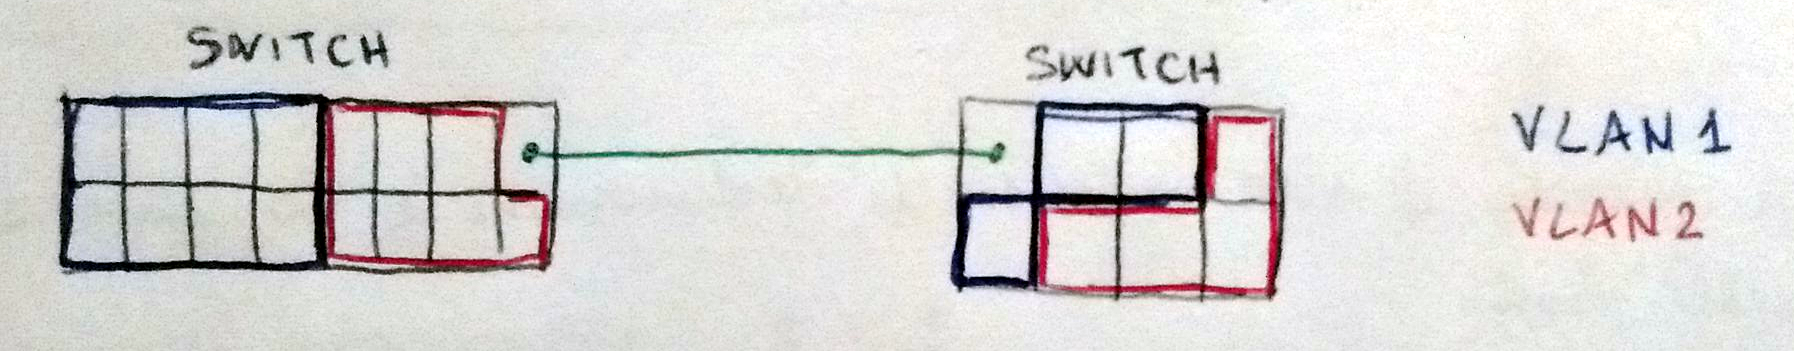
\includegraphics[width=10cm]{img/2/vlan-switch.png}
  \caption{VLAN distribuite su switch}
  \label{fig:vlan-switch}
\end{figure}

Per poter inoltrare i pacchetti alle VLAN distribuite su più switch
è necessario un collegamento tra gli switch detto \textbf{trunk},
evidenziato in verde in Figura~\ref{fig:vlan-switch}.
Per far funzionare un collegamento trunk,
occorre aggiungere un \emph{tag} al frame Ethernet, così che, una volta
giunto all'altro switch, possa essere smistato verso la giusta VLAN.

\paragraph{Frame Ethernet 802.1q per VLAN}\mbox{}\\

\begin{table}[H]
  \centering
  \begin{tabular}{| c | c | c | c | c | c | c | c | c |}\hline
  Preamble  & Dst. Addr.  & Src. Addr.  & Type & Tag Protocol ID & Tag VLAN &  Actual Data         & CRC/CRC'  \\ \hline
  64        & 48          & 48          & 16   & 16              & 12 + 3   & (46-1500)$\times$8   & 32        \\ \hline
  \end{tabular}
  \caption{Frame Ethernet 802.1q}
\end{table}

Differenze rispetto al frame Ethernet tradizionale:
\begin{itemize}
  \item Tag~Protocol~ID e Tag~VLAN: questi campi vengono inseriti
    quando il frame deve essere trasmesso tra dispositivi
    \emph{802.1q-aware} su porte \emph{tagged}, e vengono rimossi
    quando il frame viene inoltrato su una porta a cui è collegato
    un nodo \emph{802.1q-unaware}.
  \item Tag~Protocol~ID specifica il tipo di tag utilizzato. Per 802.1q
    viene usato il magic number \texttt{0x8100}
  \item Tag~VLAN specifica la VLAN sulla quale deve essere inoltrato il
    frame:
    \begin{itemize}
      \item 12 bit indicano il numero della VLAN;
      \item 3 bit indicano la priorità del frame;
      \item 1 bit indica se l'indirizzo MAC è in forma canonica.
    \end{itemize}
  \item Il CRC viene ricalcolato tenendo conto dei nuovi tag,
    ogniqualvolta questi vengono inseriti o rimossi dal frame.
\end{itemize}

\subsection{Protocollo ATM}
ATM, \emph{Asynchronous Transfer Mode}, protocollo di collegamento basato
su packet switching progettato all'inizio degli anni 1990 per integrare
diverse tipologie di servizi su di un'unica rete.

\subsubsection{Cella ATM}
Le trame del protocollo ATM non sono chiamate \emph{frame} bensì \emph{celle}.
La dimensione è ridotta per garantire un basso ritardo di pacchettizzazione,
rilevante per le applicazioni in tempo reale come la telefonia.

\begin{table}[H]
  \centering
  \begin{tabular}{| c | c |}\hline
  Header    & Payload \\ \hline
  5         & 48      \\ \hline
  \end{tabular}
  \caption{Cella ATM}
\end{table}

Tra i campi dell'header ci sono:
\begin{itemize}
  \item \textbf{VCI}, Virtual Circuit Identifier: identifica il circuito
    virtuale che interconnette il nodo mittente col nodo destinatario;
  \item \textbf{VPI}, Virtual Path Identifier: identifica il percorso
    che deve essere seguito dalla cella. Più circuiti virtuali possono
    transitare sullo stesso percorso
\end{itemize}

\subsubsection{Servizi offerti}
\begin{itemize}
  \item \textbf{CBR}: costant bitrate, per comunicazioni telefoniche
  \item \textbf{VBR}: variable bitrate, per flussi audiovisivi
  \item \textbf{ABR}: available bitrate, offre \emph{almeno} il bitrate
    richiesto
  \item \textbf{UBR}: unspecified bitrate, come Internet
\end{itemize}

\subsubsection{Chiamata}
La rete si basa sull'allocazione di un percorso virtuale tra gli switch
che simula le vecchie reti a commutazione di circuito.

\begin{enumerate}
  \item Il nodo chiamante richiede l'allocazione di un circuito verso un
    nodo destinatario. Nella chiamata, viene specificato il tipo di
    servizio;
  \item Lo switch di frontiera verifica di poter soddisfare la richiesta
    di servizio: se non può soddisfarla (per mancanza di risorse, quali
    banda o memoria), allora replica con un messaggio di errore;
    altrimenti inoltra la richiesta allo switch successivo;
  \item Gli switch successivi verificano la soddisfacibilità della
    richiesta in base alla propria disponibilità di risorse, finché non
    si giunge allo switch di frontiera del destinatario;
  \item Lo switch di frontiera del destinatario inoltra la richiesta ad
    esso, che a sua volta verifica la disponibilità delle proprie
    risorse, e, se sono sufficienti, acconsente alla comunicazione con
    il nodo mittente.
\end{enumerate}

Al termine della comunicazione, il circuito viene distrutto liberando
nuovamente risorse.

\subsubsection{Tabella di switching ATM}
Il circuito può essere identificato da un identificatore diverso nei
vari segmenti della rete, perciò ogni switch lungo il percorso possiede
una tabella di switching del tipo:
\begin{table}[H]
  \centering
  \begin{tabular}{ c c | c c }
  in-if & in-vci  & out-if  & out-vci \\ \hline
  1     & 12      & 3       & 22      \\
  2     & 63      & 1       & 18      \\
  1     & 97      & 4       & 88      \\
  ...   & ...     & ...     & ...
  \end{tabular}
  \caption{Tabella di switching per switch ATM}
\end{table}

\paragraph{Esempio}
Una cella proveniente dall'interfaccia 1 e appartenente al circuito
virtuale 12 deve essere inoltrata sull'interfaccia 3 cambiando
l'identificatore di circuito in 22; una cella proveniente
dall'interfaccia 1 a appartenente al circuito virtuale 97 deve essere
inoltrata sull'interfaccia 4 cambiando l'identificatore di circuito in
88; e così via.

\section{Livello di Rete}
Più reti locali possono essere interconnesse tra di loro in una più
grande \emph{interrete} o \emph{internet}.

Affinché la nuova rete appaia come un'unica nuova rete astratta,
occorre utilizzare un nuovo protocollo di indirizzamento.

L'indirizzamento è di tipo gerarchico.

\begin{itemize}
  \item \textbf{forwarding}, operazione di inoltro di un pacchetto da
    una porta di ingresso ad una porta di uscita, sulla base di regole
    già stabilite; questa operazione viene portata a termine grazie
    alla consultazione della \emph{tabella di forwarding} (analogia:
    svolta agli incroci)
  \item \textbf{router}, dispositivo che interconnette due o più reti;
  \item \textbf{routing}, operazione di pianificazione del percorso da
    far seguire ad un pacchetto; in seguito a questa operazione viene
    riempita la tabella di forwarding (analogia: pianificazione
    itinerario con cartina)
  \item \textbf{tabella di forwarding}, contiene le corrispondenze tra
    \emph{prefissi} e porta di collegamento di uscita;
\end{itemize}

I router di Internet, a differenza degli switch ATM, sono trasparenti al
concetto di connessione e non mantengono stato: di conseguenza,
pacchetti provenienti dallo stesso mittente e diretti allo stesso
destinatario possono venire instradati attraverso due rotte differenti.

I pacchetti vengono instradati tenendo conto solo dell'indirizzo del
destinatario.

\subsection{Router}
I pacchetti giungono al router tramite le porte di ingresso e vengono
inoltrati sull'opportuna porta di uscita da una \emph{switching fabric}
realizzata in hardware. La switching fabric viene modificata da un
programma che implementa uno o più algoritmi di routing sul
\emph{processore di instradamento}.

\begin{figure}[H]
\centering
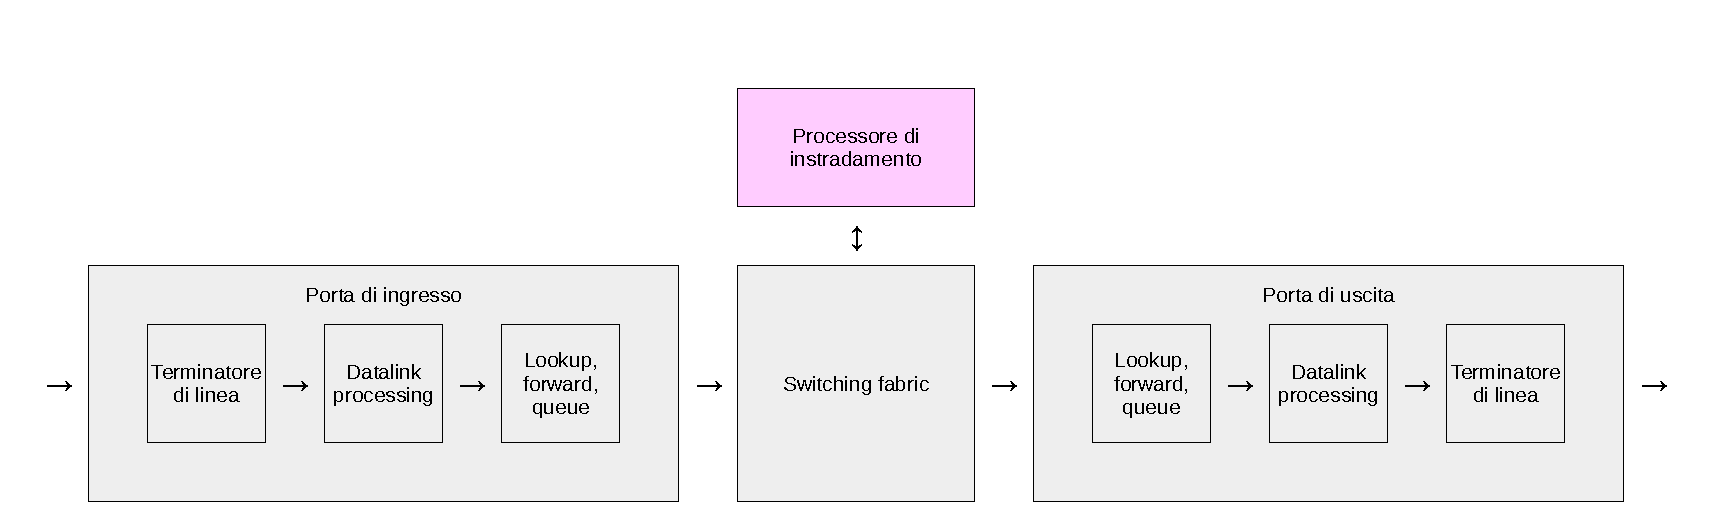
\includegraphics[width=18cm]{img/3/Router.pdf}
\caption{Architettura di un router: in viola le parti realizzate in software, in grigio quelle realizzate in hardware}
\end{figure}

\subsubsection{Struttura di una switching fabric}
\begin{table}[H]
\centering
\begin{tabular}{| c | c | c |}\hline
  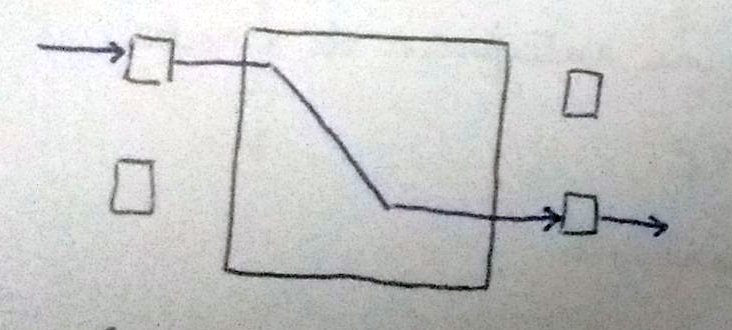
\includegraphics[width=3cm]{img/3/sf-memoria.png}  & 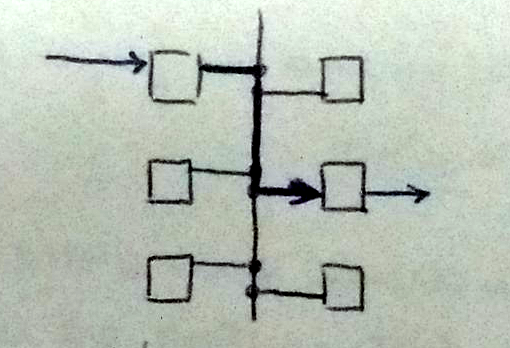
\includegraphics[width=3cm]{img/3/sf-bus.png} & 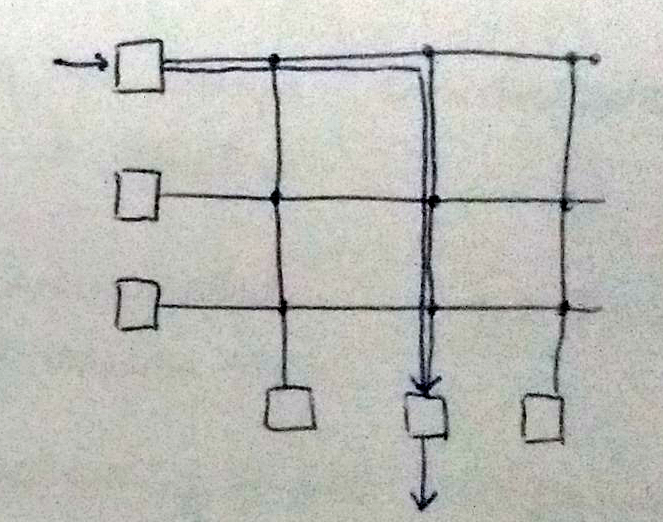
\includegraphics[width=3cm]{img/3/sf-crossbar.png} \\ \hline
  a memoria (pc comuni) & a bus & crossbar \\ \hline
\end{tabular}
\end{table}

\subsection{IP, Internet Protocol}
\subsubsection{Formato del datagramma IP}
\begin{figure}[H]
\centering
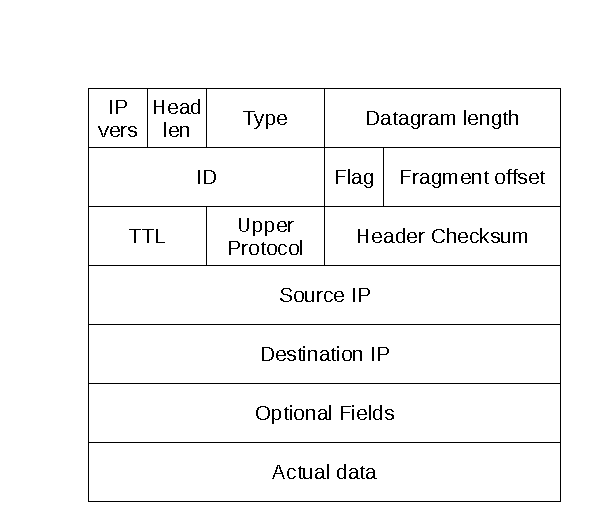
\includegraphics{img/3/IP-header.pdf}
\caption{Formato del datagramma IP. Il campo \emph{Flag} non è in scala.}
\end{figure}

\begin{itemize}
  \item \textbf{IP version}, 4 bit, attualmente può valere 4 o 6;
  \item \textbf{Header length}, 4 bit, lunghezza dell'intestazione in
    parole da 32bit; la lunghezza minima è 5 parole (20 bytes);
  \item \textbf{Type}, 8 bit, tipo del servizio, mai usato;
  \item \textbf{Datagram length}, 16 bit, lunghezza del datagramma,
    in bytes;
  \item \textbf{ID}, 16 bit, identificatore del datagramma, utilizzato
    per ricomporre datagrammi che devono essere frammentati;
  \item \textbf{Flag}, 3 bit, utilizzati per indicare la frammentazione;
  \item \textbf{Fragment offset}, 13 bit, offset del frammento trasportato
    in parole da 64 bit;
  \item \textbf{TTL}, Time To Live, 8 bit, viene decrementato ogni volta
    che il pacchetto attraversa un router; il pacchetto viene scartato
    quando TTL~==~0; costituisce un meccanismo di sicurezza per evitare
    che router mal configurati possano inoltrarsi all'infinito lo stesso
    pacchetto a vicenda, saturando la rete;
  \item \textbf{Upper protocol}, 8 bit, specifica il protocollo di livello
    di trasporto a cui deve essere consegnato il contenuto del datagramma;
  \item \textbf{Header checksum}, 16 bit, checksum dell'header;
  \item \textbf{Source IP}, 32 bit;
  \item \textbf{Destination IP}, 32 bit;
\end{itemize}

\paragraph{Frammentazione di datagramma IP}
La lunghezza massima di un datagramma IP è di 64k bytes;
L'MTU, \emph{Maximum Transmission Unit}, di un frame Ethernet è di 1500 bytes;
pertanto, può essere necessario frammentare un datagramma~IP su più frame
Ethernet in fase di trasmissione.

Nota: il datagramma può essere ulteriormente scomposto dai router
intermedi per rispettare i vincoli del particolare mezzo trasmissivo,
ma questi non lo ricompongono mai. L'onere della ricomposizione è
lasciato all'host destinatario.

\begin{table}[H]
\centering
\begin{tabular}{| c | c | c | c |}\hline
LEN = 2000  & ID = x  & OFFSET = 0  & FLAG = 0\\ \hline
\end{tabular}
\caption{Datagramma IP originale}
\end{table}
Il datagramma~IP originale trasporta 1980 bytes di informazione utile,
perciò ha una lunghezza di $1980 + 20 = 2000$ bytes.

\begin{table}[H]
\centering
\begin{tabular}{| c | c | c | c |}\hline
LEN = 1500  & ID = x  & OFFSET = 0  & FLAG = 1\\ \hline
LEN = 520   & ID = x  & OFFSET = 185  & FLAG = 0\\ \hline
\end{tabular}
\caption{Datagramma IP frammentato}
\end{table}

Un frammento può essere lungo, al massimo, 1500 bytes, perciò può
trasportare 1480 bytes di informazione utile.
Il primo frammento trasporta 1480 bytes, perciò ne devono essere
trasportati ancora 500.
Il secondo frammento ha una lunghezza di 500 bytes utili + 20 bytes di
intestazione = 520 bytes: poiché $520 < 1500$ non sono necessari altri
frammenti. L'offset di questo frammento è $1480 \div 8 = 185$.

Il FLAG~==~0 contrassegna l'ultimo frammento.

\subsubsection{CIDR, ClassLess Inter Domain Routing}
Indicazione degli indirizzi attraverso il formato
\textbf{indirizzo/sottorete}, dove:
\begin{itemize}
  \item \textit{indirizzo} è l'indirizzo dell'host, in notazione
    decimale puntata;
  \item \textit{sottorete} indica il numero di bit che costituiscono
    l'indirizzo di sottorete;
\end{itemize}
Esempio:
  192.0.2.130/25 identifica l'host 2 all'interno della rete
  192.0.2.128/25

\subsubsection{Indirizzi riservati}
\begin{table}[H]
\centering
\begin{tabular}{ c | c | l}
  Network   & Host  & Descrizione \\ \hline
  0...0     & 0...0 & utilizzato dai nodi che non possiedono un indirizzo \\
  nnn       & 0...0 & utilizzato per identificare la sottorete \emph{nnn} \\
  nnn       & 1...1 & indirizzo di broadcast della sottorete \emph{nnn}   \\
  01111111  & --    & indirizzo di loopback dell'host locale              \\
\end{tabular}
\caption{Indirizzi riservati}
\end{table}

\subsection{DHCP, Dynamic Host Configuration Protocol}
Protocollo per ottenere informazioni necessarie per la connettività:
indirizzo IP, maschera di rete, router, server DNS.
Per semplicità si sottolinea solo l'acquisizione dell'indirizzo~IP.

\subsubsection{4-ways handshake}
\begin{table}[H]
\begin{tabular}{r | c | c | c | c |}\hline
          & DHCP Discover   & DHCP Offer          & DHCP Request        & DHCP Ack            \\ \hline
src       & 0.0.0.0         & \textit{server IP}  & 0.0.0.0             & \textit{server IP}  \\
dst       & 255.255.255.255 & 255.255.255.255     & 255.255.255.255     & 255.255.255.255     \\
yiaddr    & --              & \textit{offered IP} & \textit{offered IP} & \textit{offered IP} \\
id        & \textit{id nr}  & \textit{id nr}      & \textit{id nr}      & \textit{id nr}      \\
lifetime  & --              & \textit{ttl}        & \textit{ttl}        & \textit{ttl}
\end{tabular}
\caption{Esempio di 4-way handshake}
\end{table}
Il client e il server rimangono in ascolto, rispettivamente, sulle porte UDP 68 e 67.

Osservazioni:
\begin{itemize}
  \item Un client nuovo che si connette ad una rete non possiede ancora
    un indirizzo~IP, pertanto usa come sorgente l'indirizzo 0.0.0.0;
    il client ovviamente non conosce nemmeno l'indirizzo IP del server,
    pertanto invia i messaggi all'indirizzo di broadcast; il client
    può iniziare ad utilizzare l'indirizzo~IP assegnato solo dopo il
    termine dell'handshake;
  \item Ogni messaggio contiene un identificatore univoco per permettere
    a più client e più server di distinguere i rispettivi messaggi;
  \item L'handshake fa sempre uso di indirizzi speciali (0.0.0.0 e 255.255.255.255)
    anche quando gli indirizzi specifici sono conosciuti, per permettere
    agli eventuali altri server DHCP di capire quale offerta ha accettato
    il client e quali indirizzi sono in uso;
  \item Prima dello scadere del \emph{lifetime}, il client richiede
    nuovamente un indirizzo IP, e il server eventualmente proroga il
    lifetime di quello che già possiede;
\end{itemize}

\subsection{NAT, Network Address Translation}
Meccanismo creativo a cavallo del livello 3 e 4, utilizzato per sopperire
alla carenza di indirizzi~IP, implementato sui router.

Il meccanismo consiste nella traduzione dinamica da indirizzo privato
a un indirizzo pubblico, attraverso una tabella~NAT.

Spazi di indirizzamento privati:
\begin{itemize}
  \item 10.0.0.0/8
  \item 172.16.0.0/20
  \item 192.168.0.0/16
\end{itemize}

\subsubsection{Funzionamento}
Si supponga di trovarsi nella seguente situazione:
\begin{itemize}
  \item client con indirizzo privato 10.0.0.1/24;
  \item router con indirizzo privato 10.0.0.254/24 e indirizzo pubblico
    138.76.29.7/xx;
  \item server con indirizzo pubblico 131.114.25.2/yy;
\end{itemize}

Il client desidera instaurare una connessione con il server web:
\begin{enumerate}
  \item Il client 10.0.0.1 invia un datagramma~IP al router, specificando
    il server come destinatario.\\
    \framebox{\texttt{src: 10.0.0.1,3345; dst: 131.114.25.2,80}}
  \item Il router/NAT\footnote{contravvenendo alla sua funzione propria}
    sostituisce l'indirizzo privato con il suo indirizzo pubblico, e
    (eventualmente) cambia porta sorgente; inoltre, aggiunge un nuovo
    record alla sua tabella di NAT;
    \begin{table}[H]
      \centering
      \begin{tabular}{c | c}
      LAN                 & WAN \\ \hline
      10.0.0.1,3345       & 138.76.29.7,5001  \\
      ···                 & ···
    \end{tabular}
    \end{table}
    \framebox{\texttt{src: 138.76.29.7,5001; dst: 131.114.25.2,80}}
  \item Il server risponde, pensando di interloquire con 138.76.29.7:\\
    \framebox{\texttt{src: 131.114.25.2,80; dst: 138.76.29.7,5001}}
  \item Il router/NAT sostituisce indirizzo e porta di destinazione (pubblici)
    con quelli del client (privati), utilizzando le informazioni che ha
    precedentemente memorizzato nella tabella di NAT;\\
    \framebox{\texttt{src: 131.114.25.2,80; dst: 10.0.0.1,3345}}
\end{enumerate}

Osservazione: per ogni datagramma IP viene creata una nuova entrata nella
tabella di NAT.

\subsection{Forwarding}
Tramite la conoscenza del proprio indirizzo~IP, di quello del destinatario
e della maschera di rete, un host mittente è in grado di determinare se
l'host destinatario si trova sulla sua stessa rete o no.

\begin{verbatim}
  if (MY_IP & SUBNET_MASK == DEST_IP & SUBNET_MASK) {
    // Stessa sottorete: inoltro il datagramma direttamente al destinatario
  }
  else {
    // Altra sottorete: inoltro il datagramma al router
  }
\end{verbatim}

La destinazione "fisica" di un datagramma~IP (verso l'host o il router)
viene fatta incapsulando il datagramma in un frame a livello di collegamento
che ha come destinatario l'indirizzo MAC opportuno.

Dato un indirizzo IP, per ricavare il corrispondente indirizzo a livello
di collegamento, si utilizza il protocollo ARP.

\subsection{ARP, Address Resolution Protocol}
Serve per ottenere l'indirizzo di collegamento dato l'indirizzo di rete.

ARP table: cache associativa. TTL tipico: 20 minuti.

\begin{table}[H]
\centering
\begin{tabular}{ c | c | c }
  IP                    & MAC                   & TTL                   \\ \hline
  IP\textsubscript{1}   & MAC\textsubscript{1}  & TTL\textsubscript{1}  \\
  ···               & ···               & ···               \\
  IP\textsubscript{n}   & MAC\textsubscript{n}  & TTL\textsubscript{n}  \\
\end{tabular}
\end{table}

Richiesta ARP:

\framebox{\texttt{A: src: MAC\textsubscript{A}; dst: FF.FF.FF.FF.FF.FF; payload: IP\textsubscript{B}}}\\
\framebox{\texttt{B: src: MAC\textsubscript{B}; dst: MAC\textsubscript{A}; payload: IP\textsubscript{B}}}

\subsection{ICMP, Internet Control Message Protocol}
Segnalazione di errori e anomalie. Esempi:
\begin{itemize}
  \item Echo request
  \item Echo reply
  \item TTL expired
  \item Host/Network/Port unreachable
  \item Unknown layer-4 protocol
  \item ···
\end{itemize}

Messaggio ICMP:
\begin{tabular}{| c | c | c |}\hline
  tipo  & codice  & ID\textsubscript{PKG} \\ \hline
\end{tabular}

ID\textsubscript{PKG} identifica il pacchetto che ha originato l'errore,
ed è composto dal suo header e dai primi 8 bytes del payload.

\subsection{IPv6, Internet Protocol versione 6}
\begin{figure}[H]
\centering
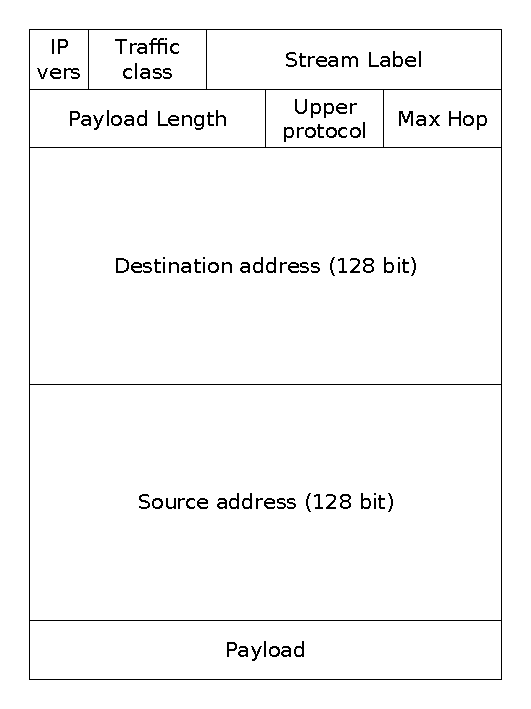
\includegraphics{img/3/ipv6-head.pdf}
\caption{Formato del datagramma IPv6, in scala}
\end{figure}

\subsubsection{Considerazioni sul datagramma IPv6}
\begin{itemize}
  \item Lunghezza intestazione ottimizzata a 40 byte, per semplificate
    e quindi velocizzare il processo di forwarding;
  \item Possibilità di etichettare i flussi e assegnare una classe di
    priorità ai singoli pacchetti, per permettere l'introduzione di
    differenti scaglioni di QoS.
  \item Eliminati campi opzionali;
  \item Eliminato controllo di integrità: viene delegato ai protocolli
    a livello di collegamento e di trasporto;
  \item Eliminata frammentazione: viene delegata all'host sorgente,
    che viene avvertito dell'eccessiva lunghezza del datagramma per
    mezzo di un messaggio ICMP;
\end{itemize}

\subsubsection{Considerazioni sulla transizione da IPv4 a IPv6}
\begin{itemize}
  \item \textbf{Dual-Stacking}: tecnica che prevede l'utilizzo di
  dispositivi di rete in grado instradare sia datagrammi IPv4 che
  datagrammi IPv6. Tutti i nuovi dispositivi IPv6 in commercio sono
  retrocompatibili con IPv4 e quindi dual-stack\footnote{a parte il mio
  router della Telecom}
  \item \textbf{Tunnelling}: incapsulamento di un datagramma IPv6 nel
  payload di un datagramma IPv4, tramite un relay terzo. Viene
  utilizzata soprattutto nel caso in cui si disponga già di connettività
  IPv4.
\end{itemize}

\subsection{Algoritmi di routing}
Terminologia:
\begin{itemize}
  \item \textbf{Autonomous System}, o \emph{AS}, è una rete di reti
    facente parte di Internet e gestita da un'unica
    organizzazione;\footnote{per esempio, la rete del GARR}
  \item \textbf{Advertisement}, messaggio pubblicitario il cui scopo è
    informare i router vicini di un cambiamento nella topologia della
    rete (creazione, distruzione o cambiamento del costo dei collegamenti)
\end{itemize}

Tipologie di algoritmi:
\begin{itemize}
  \item \textbf{Link State}: ogni router dispone di una rappresentazione
    completa dell'\emph{AS} a cui è collegato; ha una visione d'insieme
    della rete;
  \item \textbf{Distance Vector}: ogni router dispone solo di un vettore
    contenente i costi dei percorsi per raggiungere gli altri router
    attraverso i suoi vicini; ha una visione molto limitata della rete;
\end{itemize}

\subsubsection{Protocolli di routing intra-AS}
Permettono di stabilire il percorso a costo minimo per raggiungere
i router all'interno dello stesso AS.

\paragraph{RIP, Routing Information Protocol}\mbox{}\\
Implementato da un'applicazione che usa il protocollo di trasporto UDP
e porta 520.
\begin{itemize}
  \item Approccio di tipo \emph{distance vector};
  \item Ogni collegamento ha un costo fisso unitario;
  \item Massimo numero di hop consentito: 15;
  \item Massimo numero di sottoreti collegabili: 25;
  \item Periodo di advertisement: 30s;
  \item Se non viene trasmesso un advertisement su di un collegamento
    per più di 180s, il collegamento viene contrassegnato come
    inutilizzabile;
\end{itemize}

\subparagraph{Routing Table RIP}
Accorpa forwarding table e distance vector in un'unica struttura:
\begin{table}[H]
\centering
\begin{tabular}{ c | c | c }
Destination Network & Interface & Cost  \\ \hline
··· & ··· & ··· \\
··· & ··· & ··· \\
\end{tabular}
\caption{Routing and forwarding table per protocollo RIP}
\end{table}

\paragraph{OSPF, Open Shortest Path First}\mbox{}\\
Implementato a livello 4 dello stack (ha un proprio numero
identificativo di protocollo di livello 4, al pari di TCP e UDP).
\begin{itemize}
  \item approccio di tipo \emph{link state};
  \item inoltro periodico del link state tramite \emph{flooding};
  \item periodo di advertisement: non appena viene rilevato un
    cambiamento nel grafo della rete, o al massimo ogni 30 minuti;
  \item offre meccanismo di autenticazione (advertisement firmati);
  \item permette l'uso di più percorsi con lo stesso costo verso
    un'unica destinazione;
  \item permette l'uso di costi diversificati sui vari collegamenti;
  \item permette una divisione gerarchica dei router dell'AS;
\end{itemize}

\subsubsection{Protocolli di routing inter-AS}
Permettono di stabilire il percorso a costo minimo all'interno di un AS
per raggiungere destinazioni esterne a tale AS.

Usano un approccio detto "patata bollente": il pacchetto non segue il
percorso a costo minimo in assoluto, ma segue il percorso a costo minimo
all'interno del proprio AS, dopodiché viene consegnato all'AS esterno e
il problema di ricerca del percorso a costo minimo viene così eliminato.

\paragraph{BGP, Border Gateway Protocol}\mbox{}\\
Implementato come applicazione che usa il protocollo di trasporto TCP.

Funzionamento (a grandi linee):
\begin{itemize}
  \item Il router di bordo di un AS\textsubscript{1} invia un
    advertisement contenente i prefissi che è in grado di instradare ai
    router di bordo degli AS con cui è collegato;
  \item I router di bordo degli AS esterni decidono se "fidarsi" delle
    informazioni contenute nell'advertisement in base alle politiche
    aziendali interne e agli accordi commerciali che gli enti che
    gestiscono gli AS hanno stipulato.
\end{itemize}

Messaggio BGP:
\begin{itemize}
  \item \textbf{prefisso}: indica la sottorete che il router di bordo è
    in grado di raggiungere;
  \item \textbf{attributi}:
    \begin{itemize}
      \item quali o quanti AS devono essere attraversati per raggiungere
        il determinato prefisso;
      \item router che ha propagato per primo l'informazione (utilizzato
        dai router all'interno dell'AS per sapere a quale router di
        bordo instradare i pacchetti destinati ad AS esterni)
    \end{itemize}
\end{itemize}

\section{Livello di Trasporto}
\subsection{Generalità}
I pacchetti a livello di trasporto vengono definiti \emph{segmenti}.

\subsubsection{Servizi offerti}
\begin{itemize}
  \item Multiplexing / Demultiplexing: uso di un solo collegamento tra
    host a livello di rete per realizzare più collegamenti virtuali tra
    processi;
  \item Reliable data transfer: controllo di integrità dei dati
    trasmessi;
  \item Flow control: controllo della velocità di trasmissione per
    evitare congestione presso un host destinatario lento;
  \item Congestion control: controllo della velocità di trasmissione
    per evitare congestione nel core della rete (e nei dispositivi
    di rete intermedi);
  \item Connection: mantenimento dello stato del flusso;
\end{itemize}

\begin{table}[H]
\centering
\begin{tabular}{| c | c | c | c | c | c |}\hline
  Protocollo  & Multiplexing  & Connection  & Reliability & Flow Control  & Congestion Control  \\ \hline
  TCP         & sì            & sì          & sì          & sì            & sì                  \\ \hline
  UDP         & sì            & no          & no          & no            & no                  \\ \hline
\end{tabular}
\caption{Riepilogo dei servizi offerti da due protocolli a livello di trasporto}
\end{table}

\subsection{UDP, User Datagram Protocol}
\subsubsection{Demultiplexing}
I segmenti vengono distinti in base alla tupla (IP\textsubscript{dst}, port\textsubscript{dst}).
IP\textsubscript{src} e port\textsubscript{src} non sono rilevanti al fine del demultiplexing.

\begin{figure}[H]
  \centering
  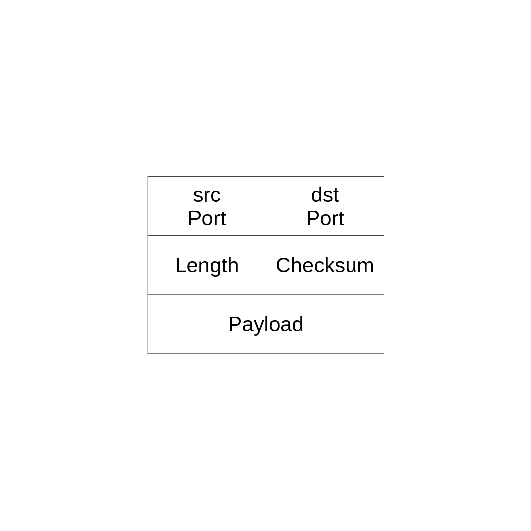
\includegraphics[width=6cm]{img/4/udp-head.pdf}
  \caption{Formato del segmento UDP}
\end{figure}

\subsection{TCP, Transmission Control Protocol}
\subsubsection{Demultiplexing}
I segmenti vengono distinti in base alla tupla (IP\textsubscript{src}, port\textsubscript{src}, IP\textsubscript{dst}, port\textsubscript{dst}).

\subsubsection{Formato del segmento}
\begin{figure}[H]
  \centering
  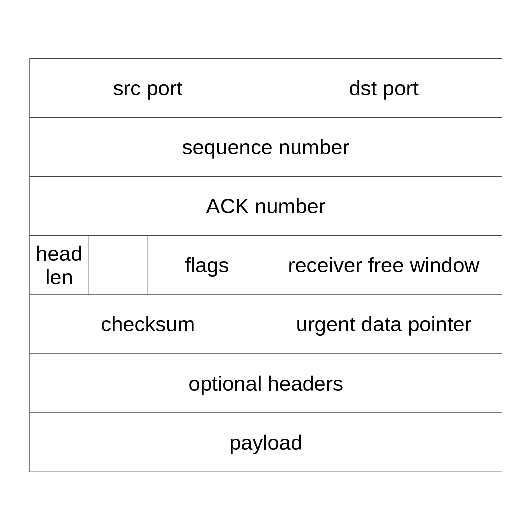
\includegraphics[width=6cm]{img/4/tcp-head.pdf}
  \caption{Formato del segmento TCP}
\end{figure}

\begin{itemize}
  \item \textbf{src port, dst port}: porta sorgente e porta destinataria;
  \item \textbf{sequence number}: indice del primo byte del pacchetto;
  \item \textbf{ACK number}: indice dell'ultimo byte correttamente ricevuto;
    si osservi che il protocollo è full duplex;
  \item \textbf{header length}: lunghezza dell'header in parole da 32bit;
  \item \textbf{Flags}: indormazioni aggiuntive sul segmento; nella figura
    non è in scala; alcuni bit di flag non sono rappresentati;
  \begin{itemize}
    \item \textbf{URG}: urgent segment, quasi mai usato;
    \item \textbf{ACK}: ack valid, indica se il campo \emph{ACK number} è significativo;
    \item \textbf{PSH}: push, mai usato;
    \item \textbf{RST}: reset, resetta la connessione;
    \item \textbf{SYN}: attivazione della connessione;
    \item \textbf{FIN}: terminazione della connessione;
  \end{itemize}
  \item \textbf{receiver free window}: spazio libero nel buffer del
    ricevitore;
  \item \textbf{checksum}: checksum in blocchi da 16bit;
  \item \textbf{urgent data pointer} e \textbf{optional headers} mai usati;
  \item \textbf{payload}: i dati effettivi;
\end{itemize}

\subsubsection{Attivazione connessione: 3-way handshake}
\begin{figure}[H]
\centering
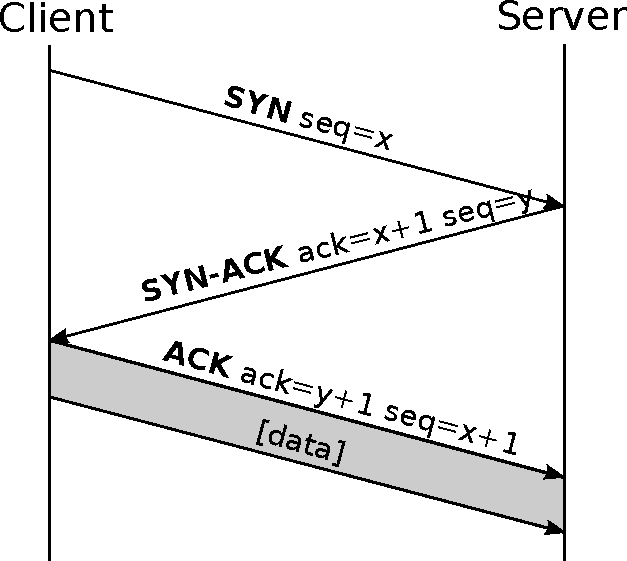
\includegraphics[width=8cm]{img/4/tcp-3way-hs.pdf}
\end{figure}

Osservazioni:
\begin{itemize}
  \item I numeri di sequenza \emph{x} e \emph{y} vengono scelti casualmente;
    La scelta casuale diminuisce la probabilità che pacchetti ritardatari
    di una connessione chiusa che giungono al destinatario dopo che è stata
    instaurata una nuova connessione, vengono scambiati per segmenti appartenenti
    alla nuova connessione;
  \item I pacchetti con il flag SYN settato non devono contenere dati nel payload;
\end{itemize}

\subsubsection{Terminazione connessione: 4-way handshake}
\begin{figure}[H]
\centering
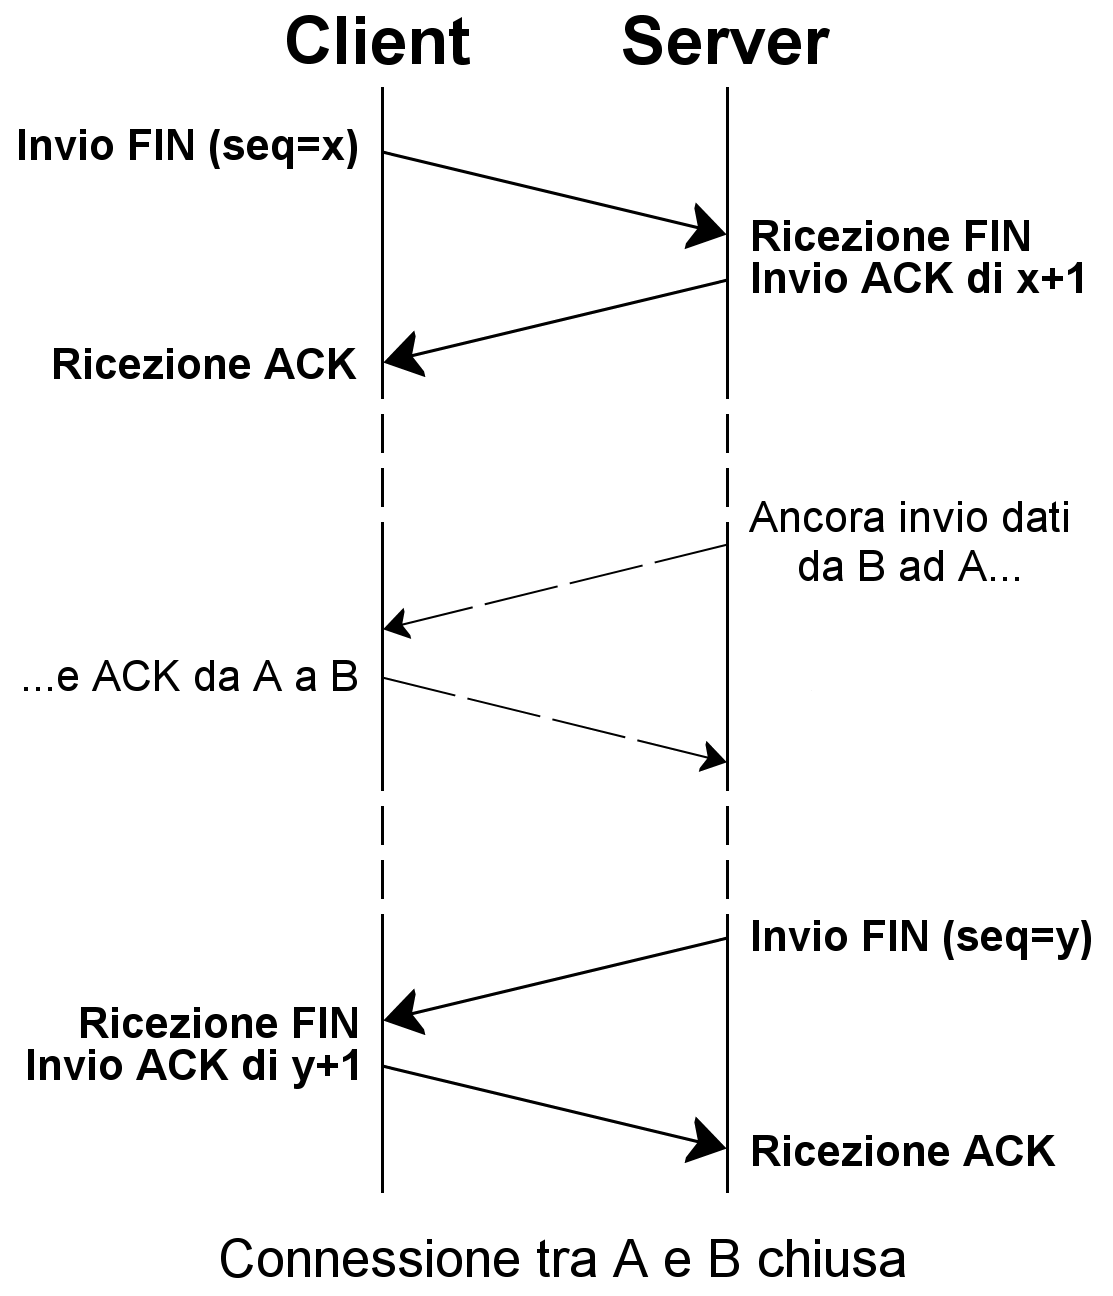
\includegraphics[width=8cm]{img/4/tcp-4way-hs.png}
\end{figure}

\subsubsection{Stima del RTT tramite media esponenziale mobile}
Simboli utilizzati:
\begin{itemize}
  \item \textbf{RTT}, Round Trip Time;
  \item \textbf{ERTT}, Estimated Round Trip Time;
\end{itemize}

$$ ERTT_1 = RTT_0 $$
$$ ERTT_2 = \alpha RTT_1 + (1 - \alpha) RTT_0 $$
$$ ERTT_3 = \alpha RTT_2 + \alpha(1 - \alpha) RTT_1 + (1 - \alpha)^2 RTT_0 $$
$$ \cdot \cdot \cdot  $$
$$ ERTT_{n + 1} = \alpha RTT_n + \alpha(1 - \alpha) RTT_{n - 1} + (1 - \alpha)^2 RTT_{n - 2} + \cdot \cdot \cdot + (1 - \alpha)^n RTT_0 $$
$$ ERTT_{n + 1} = \alpha RTT_n + (1 - \alpha) (\alpha RTT_{n - 1} + (1 - a)^{2} RTT_{n - 2} + \cdot \cdot \cdot + (1 - \alpha)^{n - 1} RTT_0) $$
$$ ERTT_{n + 1} = \alpha RTT_n + (1 - \alpha) ERTT_{n} $$

\clearpage
\printbibliography[heading=bibintoc]

\end{document}
